
\chapter{Elementary Regression}


\section{Example}

Here's what I would do to begin a regression exercise. I'm using the
dataset ``Prestige'' that is in the car package for R.

\inputencoding{latin9}\begin{lstlisting}[breaklines=true]
library(car)

pdf(file="car.inc.ed.pdf", height=5,width=5, onefile=F, paper="special")
plot(income~education, xlab="Education", ylab="Income", main="", data=Prestige)
dev.off()
\end{lstlisting}
\inputencoding{utf8}

That plot is presented in the top panel in Figure \ref{fig:Income-DependsonEduc}. 

A regression model \citet{gelman_bayesian_2003}can be fitted to that
scatterplot with R's lm function.

\inputencoding{latin9}\begin{lstlisting}
mymod <- lm(income~education, data=Prestige)
\end{lstlisting}
\inputencoding{utf8}

mymod is an ``object'', a complicated structure that contains a
great deal of information. Observe:

\inputencoding{latin9}\begin{lstlisting}
attributes(mymod)
$names  
[1] "coefficients"  "residuals"     "effects"       "rank"           
[5] "fitted.values" "assign"        "qr"            "df.residual"    
[9] "xlevels"       "call"          "terms"         "model"        
$class 
[1] "lm" 
\end{lstlisting}
\inputencoding{utf8}

We can access values from mymod by 2 methods. 
\begin{enumerate}
\item Direct access 


\inputencoding{latin9}\begin{lstlisting}
> mymod$coefficients
> mymod$coefficients
(Intercept)   education 
 -2853.5856    898.8128 
\end{lstlisting}
\inputencoding{utf8}

\item Or by ``accessor'' methods.
\end{enumerate}
\inputencoding{latin9}\begin{lstlisting}
> coef(mymod)
(Intercept)   education 
 -2853.5856    898.8128 
\end{lstlisting}
\inputencoding{utf8}

Some values are needed so regularly that a ``summary'' method is
written to gather and summarize them.

\inputencoding{latin9}\begin{lstlisting}
> summary(mymod)
Call:
lm(formula = income ~ education, data = Prestige)
Residuals:
     Min       1Q   Median       3Q      Max 
-5493.20 -2433.80   -41.92  1491.50 17713.14 
Coefficients:
            Estimate Std. Error t value Pr(>|t|)    
(Intercept)  -2853.6     1407.0  -2.028   0.0452 *  
education      898.8      127.0   7.075 2.08e-10 ***
---
Signif. codes:  0 '***' 0.001 '**' 0.01 '*' 0.05 '.' 0.1 ' ' 1 
Residual standard error: 3483 on 100 degrees of freedom
Multiple R-squared: 0.3336,	Adjusted R-squared: 0.3269 
F-statistic: 50.06 on 1 and 100 DF,  p-value: 2.079e-10 
\end{lstlisting}
\inputencoding{utf8}

There are some functions to make more beautiful tables that are closer
to the needs of journals. Years ago, I wrote a function called ``outreg''
and it would make a nice looking table. You can use that if you want,
but if I were you, I would use the regression tables from either of
these packages for R: ``memisc'' or ``apsrtable''. Since I already
have memisc installed, I will demonstrate that:

\inputencoding{latin9}\begin{lstlisting}
> library(memisc)
> toLatex(mtable(mymod))
\end{lstlisting}
\inputencoding{utf8}

The \LaTeX{} code can be pasted into a document in the same way that
we handled cross tabulation tables. Please see Table \ref{tab:My-Regression-Table}

\begin{table}


\begin{centering}
\caption{My Regression Table\label{tab:My-Regression-Table}}

\par\end{centering}

\begin{centering}
\begin{tabular}{lD{.}{.}{7}}
\toprule
(Intercept)    & -2853.586^{*}  \\
               &  (1407.039)    \\
education      &   898.813^{***}\\
               &   (127.035)    \\
\midrule
R-squared      &          0.334 \\
adj. R-squared &          0.327 \\
sigma          &       3483.378 \\
F              &         50.060 \\
p              &          0.000 \\
Log-likelihood &       -975.609 \\
Deviance       & 1213392025.001 \\
AIC            &       1957.218 \\
BIC            &       1965.093 \\
N              &        102     \\
\bottomrule
\end{tabular}
\par\end{centering}

\centering{}
\end{table}


Observe:

The function ``predict'' can be used to obtain predicted values
for example values of the input. One specifies a ``newdata'' option
which must be a data frame, but we can create the new dataframe ``on
the fly'' without too much trouble. 

\inputencoding{latin9}\begin{lstlisting}
> predict(mymod, newdata=data.frame(education=c(8,9,10,11,12)))
       1        2        3        4        5 
4336.917 5235.730 6134.543 7033.356 7932.169 
\end{lstlisting}
\inputencoding{utf8}

Sometimes we want to plot the predictive line in the model, and that
can be done in a variety of ways. One way is to find some points and
then use them with the lines function.

\inputencoding{latin9}\begin{lstlisting}
> range(Prestige$education)
[1]  6.38 15.97
> predict(mymod, newdata=data.frame(education=range(Prestige$education)))
        1         2 
 2880.840 11500.456 
> X1 <- range(Prestige$education)
> Y1 <- predict(mymod, newdata=data.frame(education=range(Prestige$education)))
> lines(X1,Y1)
\end{lstlisting}
\inputencoding{utf8}

That adds a line to the figure, as seen in the bottom panel.

Because it is very common to add a regression line to a plot, the
R function abline has been customized to do this for us automatically
if you give it a regression object. The following commands were the
ones I actually used to produce the figure. 

\inputencoding{latin9}\begin{lstlisting}[breaklines=true]
pdf(file="car.inc.ed-fit.pdf" height=5, width=5, onefile=F, paper="special")
plot(income~education, xlab="Education", ylab="Income", main="",data=Prestige)
abline(mymod)
dev.off()
\end{lstlisting}
\inputencoding{utf8}

I went to the trouble of illustrating the ``old fashioned'' way
because I think it is possible to become too dependent on simplifying
functions, especially when they don't do exactly what you want.

\begin{figure}
\begin{centering}
\subfloat[A Scatterplot]{\begin{centering}
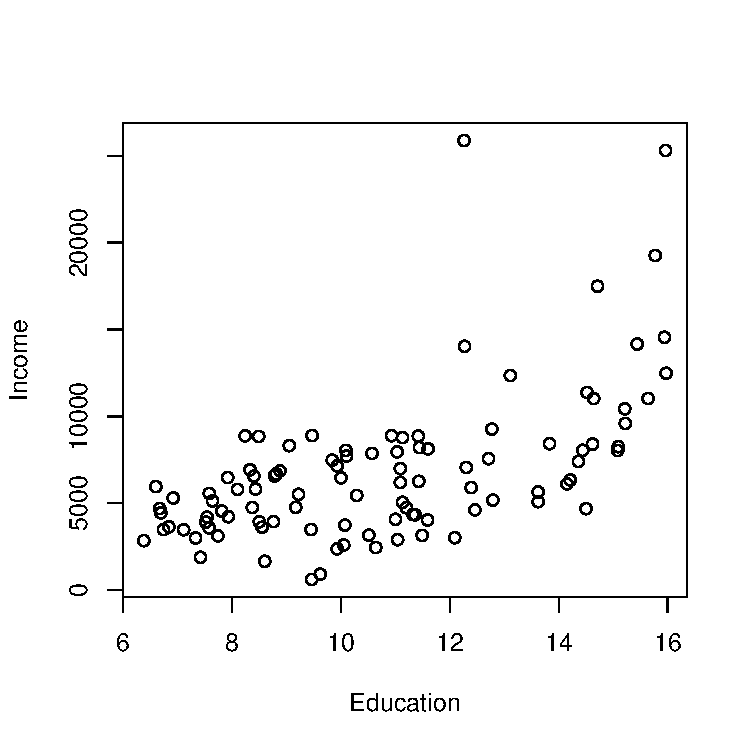
\includegraphics[width=4in]{Chapter2/importfigs/carinced}
\par\end{centering}

}
\par\end{centering}

\begin{centering}
\subfloat[Add the ``regression line'']{\begin{centering}
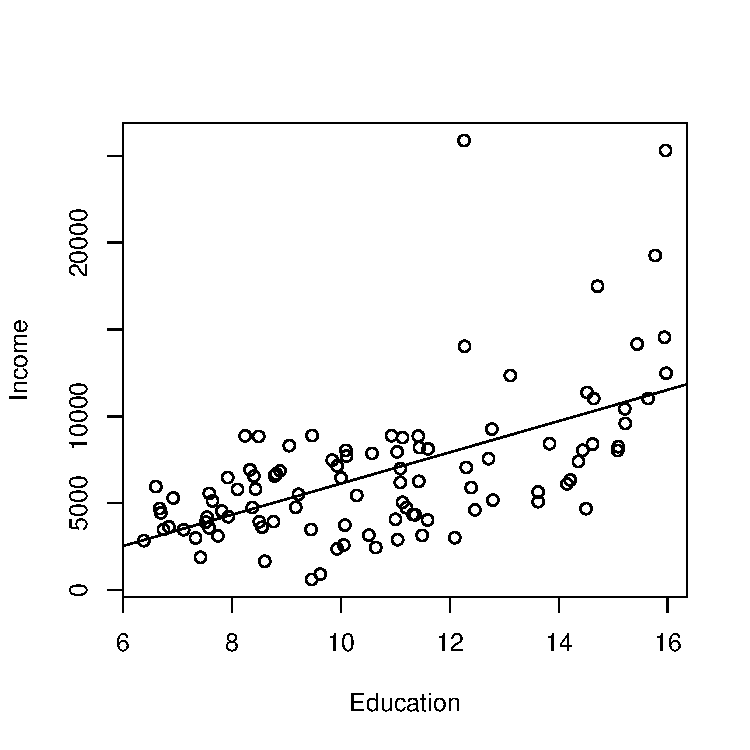
\includegraphics[width=4in]{Chapter2/importfigs/carinced-fit}
\par\end{centering}

}
\par\end{centering}

\caption{Income Depends on Education\label{fig:Income-DependsonEduc}}
\end{figure}

